%!TEX root = ../main.tex
\section{Multivariate dependence in univariate residuals} % (fold)
\label{sec:multivariate_dependence}
% explain the logic in what we are doing, that there might still be dependence in what looks like white noise residuals
After the univariate modeling of returns in ARMA-GARCH models, we find that the ARMA-GARCH residuals look like white noise, with no serial correlation or ARCH effects. However, when considered jointly, we find that there is substantial dependence remaining in the residual series -- as will be shown in this section, correlation is non-zero and time-varying, and there is tail dependence between the residual series. 

Therefore, we do not use returns directly in the multivariate analysis, as significant parts of the dependence can be removed by univariate models alone. Instead, we use the residuals from the ARMA-GARCH models. The intuition behind this is that we do not want to confuse multivariate dependency in returns with what are in fact just predictable effects that can be understood on the univariate level alone.

Our philosophy, which is in line with the copula methodology, is to try to sanitize the data as far as possible on the univariate level. Then, any dependence left in the residuals can be attributed to multivariate dependence.

\subsection{Threshold correlations}
\label{subsec:threshold_corr}
% method
Threshold (or exceedance) correlations have previously been used to highlight the asymmetric dependence structure of i.a. country equity indices~\autocite{LonginSolnik2001}, portfolios by industry, size, value and momentum~\autocite{AngChen2002} and factor strategies~\autocite{ChristoffersenLanglois2013}. The following analysis is still new as it adds the factors investment (CMA) and profitability (RMW). We follow~\textcite{ChristoffersenLanglois2013} definition of threshold correlation
\begin{align}
    ThCorr(r_i, r_j) = 
    \begin{cases} 
        Corr\Big(r_i, r_j \,|\, r_i < F_i^{-1}(p), r_j < F_j^{-1}(p)\Big)  & \text{for } p < 0.5 \\
        Corr\Big(r_i, r_j \,|\, r_i \geq F_i^{-1}(p), r_j \geq F_j^{-1}(p)\Big)  & \text{for } p \geq 0.5
    \end{cases}
\end{align}
where $F_i^{-1}(p)$ the empirical quantile of $r_i$ at percentile $p$. 

Graphically, threshold correlation are understood as the standard correlation estimate in more and more distant parts of the first and third quadrant as $p$ approaches either zero or unity. This subsetting of data is illustrated in \autoref{fig:illustrate_threshold}. 

\begin{figure}[H]
  \caption{Threshold correlation explained. Mkt-RF - HML factor pair}
  \label{fig:illustrate_threshold}
  %\toprule
  \centering
  \begin{minipage}{\textwidth}
  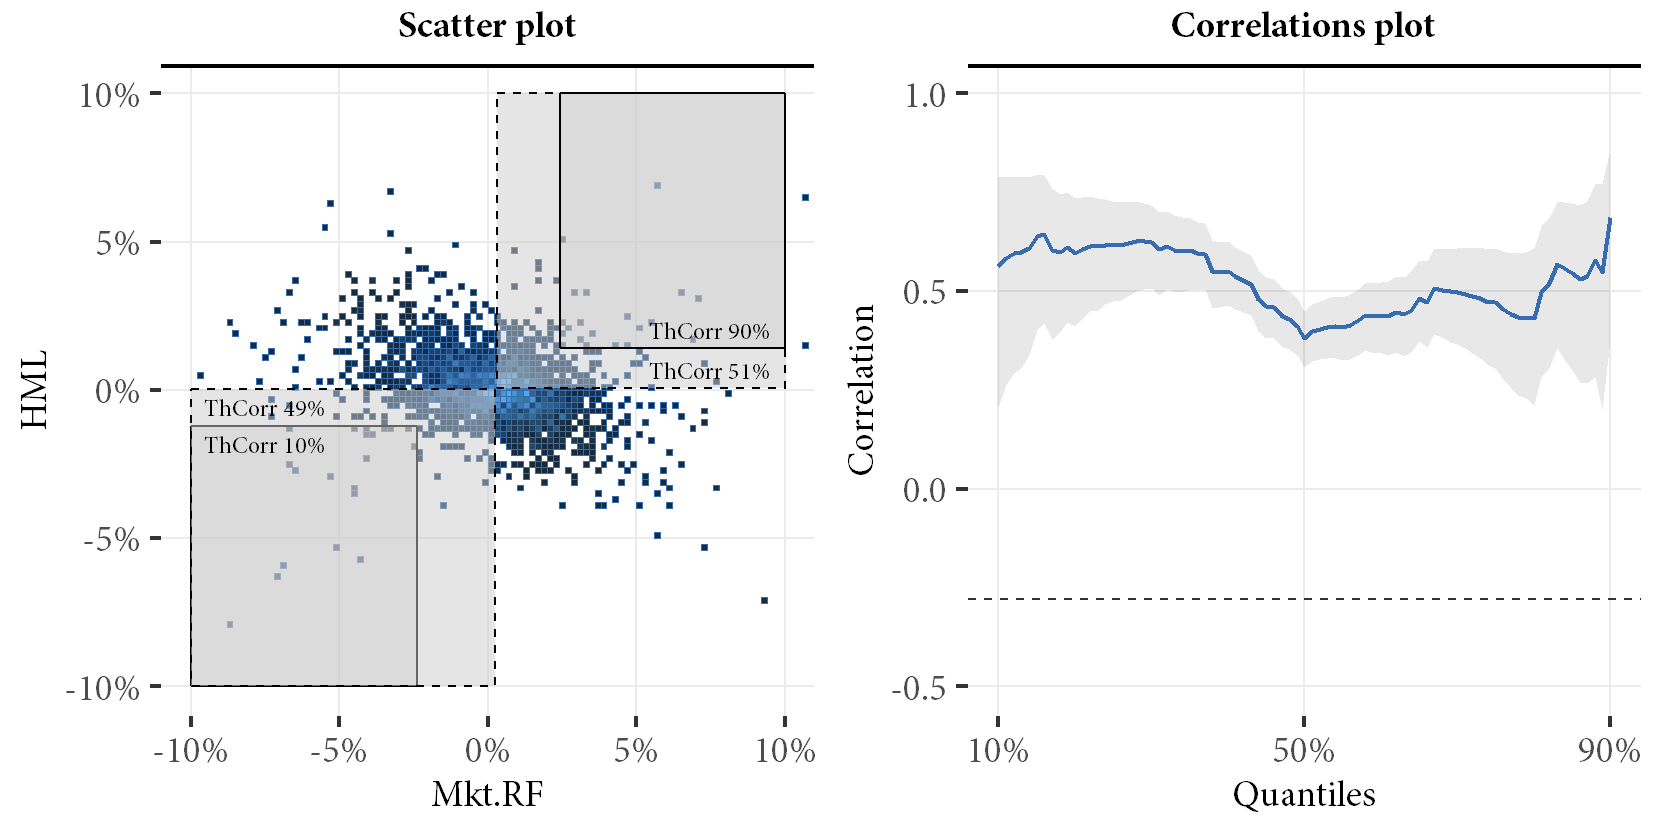
\includegraphics[scale=1]{graphics/threshold_explain_ret.png}  
  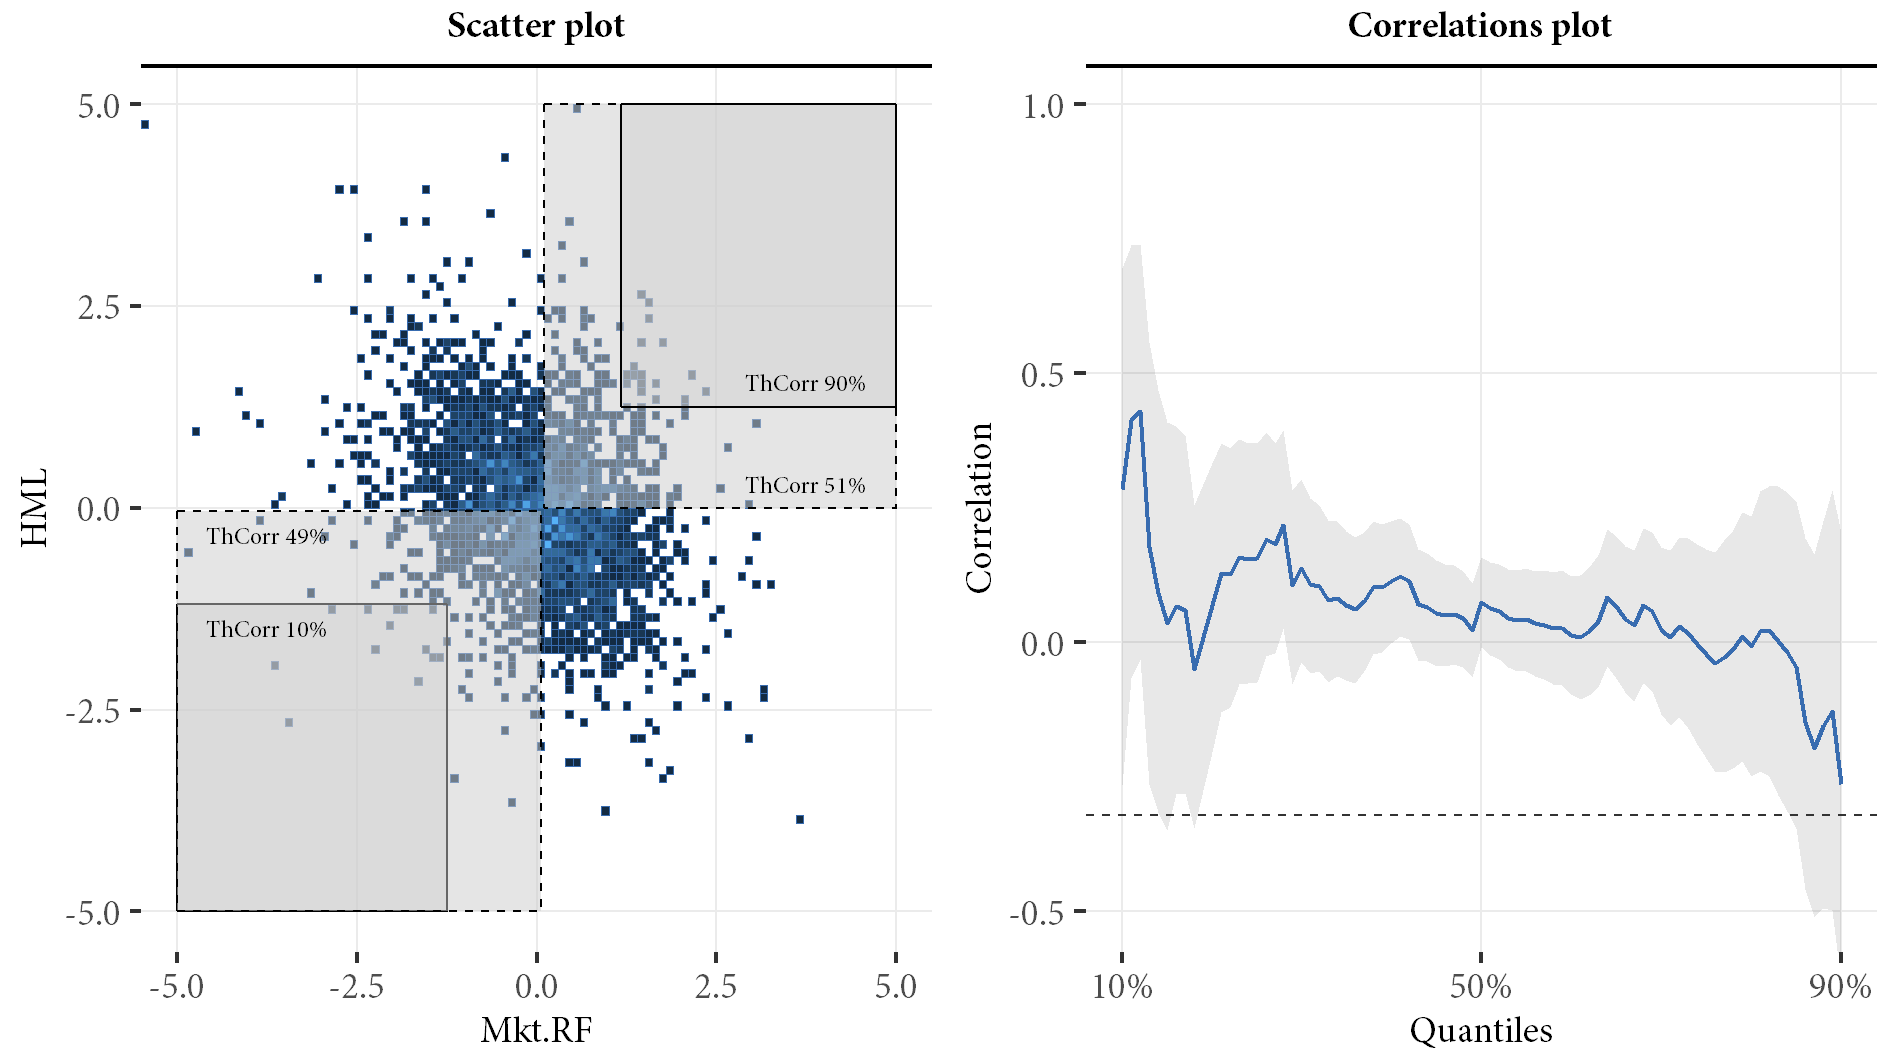
\includegraphics[scale=1]{graphics/threshold_explain_res.png}  
  %\bottomrule
  \vspace{3mm}
  \footnotesize
  Threshold correlation plots with 95\% confidence bounds. Unconditional correlation given by the dashed line. The upper two panels use log return data and the lower two panels use ARMA-GARCH residuals from the chosen models. Weekly data 1963-2016
  \end{minipage}
\end{figure}

In the left hand plots, we see the scatter of returns and ARMA-GARCH residuals of Mkt-RF and HML respectively, and how $p$, found on the x axis of the right hand plot, determines the subset of data that is included in the correlation calculation. Note that the further away from the median we get, the more uncertain the point estimate of the correlation coefficient becomes, as fewer observations are available. For the 49\% and 51\% points, estimates are much more precise as essentially half the data set is available. We also note that the standard correlation, given by the dashed line in the right hand plot, is clearly negative, while threshold correlations in the first and third quadrants are significantly more positive, which shows the usefulness of this analysis; not taking threshold correlations into account provides a vaguer picture of the dependence structure.

Although threshold correlations are nothing but linear correlation coefficients for a subset of the data, they do provide an intuitive measure of tail dependence -- how correlated are returns in bad times? And does this differ from the correlation in good times? Ceteris paribus, assets pairs with weaker or negative threshold correlation as $p \rightarrow 0$ are better diversified, as they have less tendency to coincide in extreme negative realizations. [ADD SOMETHING ABOUT Between two normal distributed variables you expect /\-shape (for positively correlated variables).]

\begin{figure}[H]
  \caption{Threshold correlations on ARMA-GARCH residuals. Page 1/2}
  \label{fig:threshold1}
  %\toprule
  \centering
  \begin{minipage}{\textwidth}
  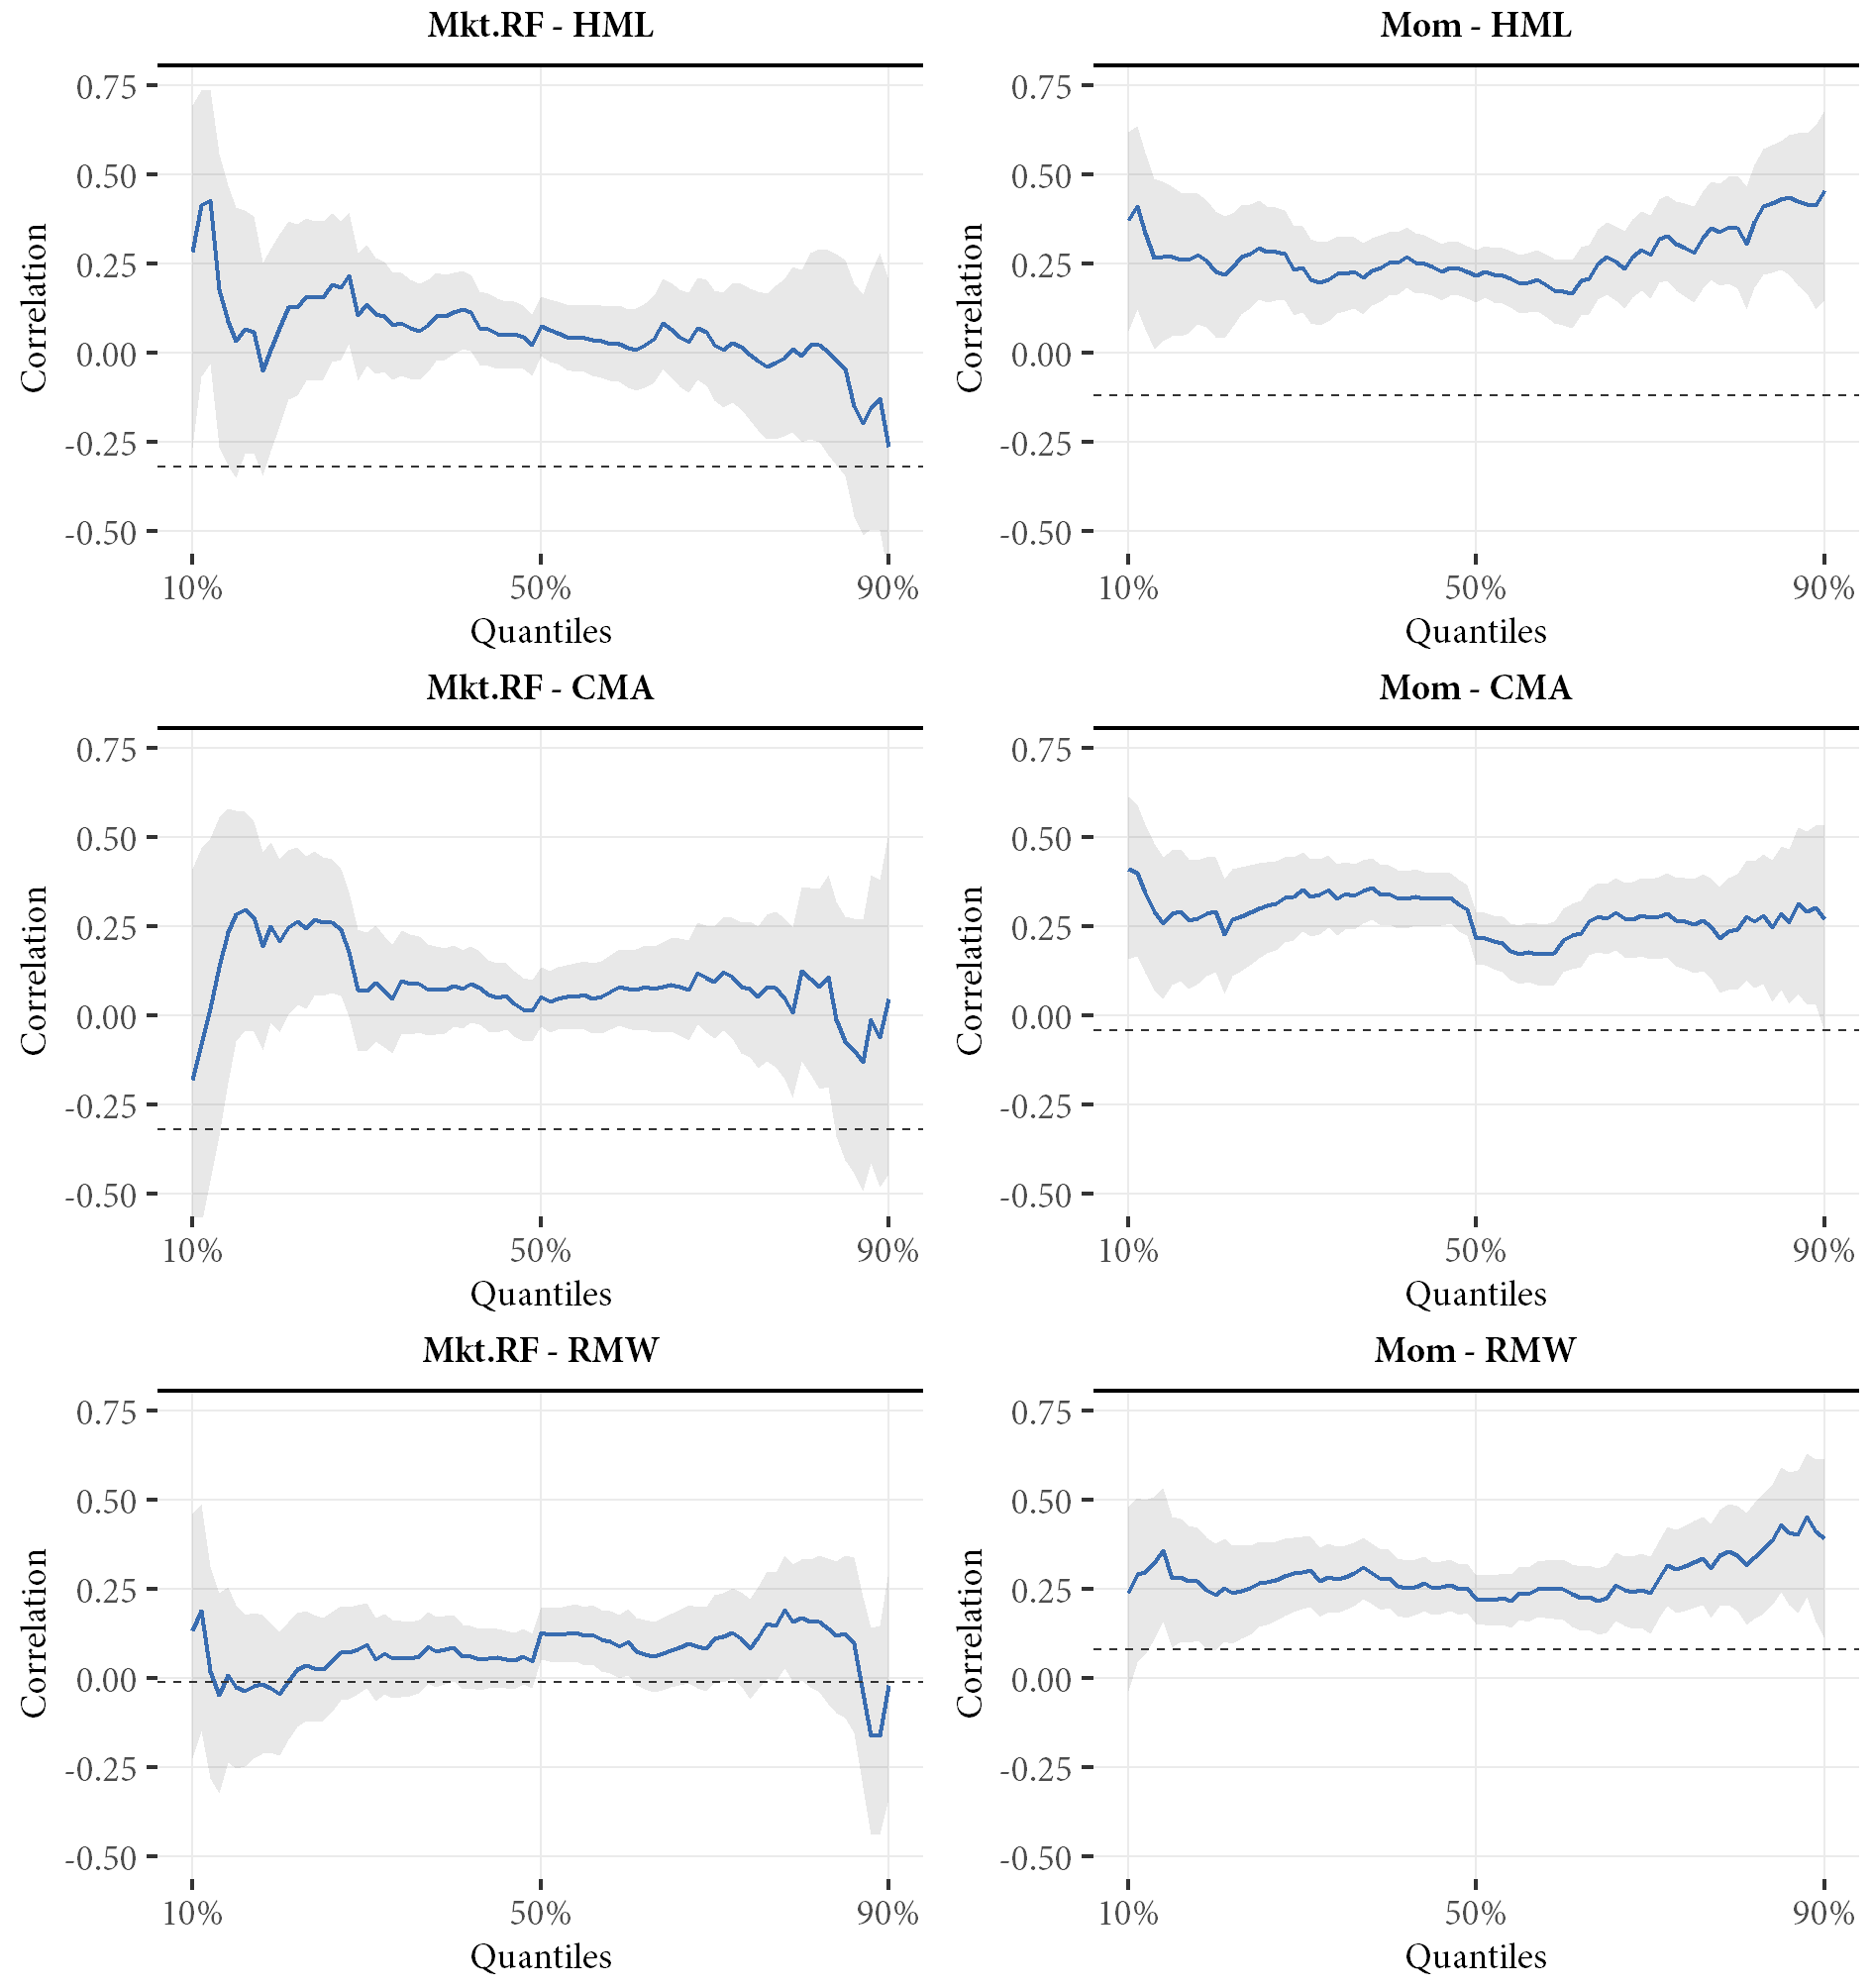
\includegraphics[scale=1]{graphics/threshold1.png}  
  %\bottomrule
  \vspace{3mm}
  \footnotesize
  Threshold correlation plots with 95\% confidence bounds. Correlation pairs in graph titles. Unconditional correlation given by the dashed line. Weekly ARMA-GARCH residuals from the chosen models, all data 1963-2016
  \end{minipage}
\end{figure}
\begin{figure}[H]
  \caption{Threshold correlations on ARMA-GARCH residuals. Page 2/2}
  \label{fig:threshold2}
  %\toprule
  \centering
  \begin{minipage}{\textwidth}
  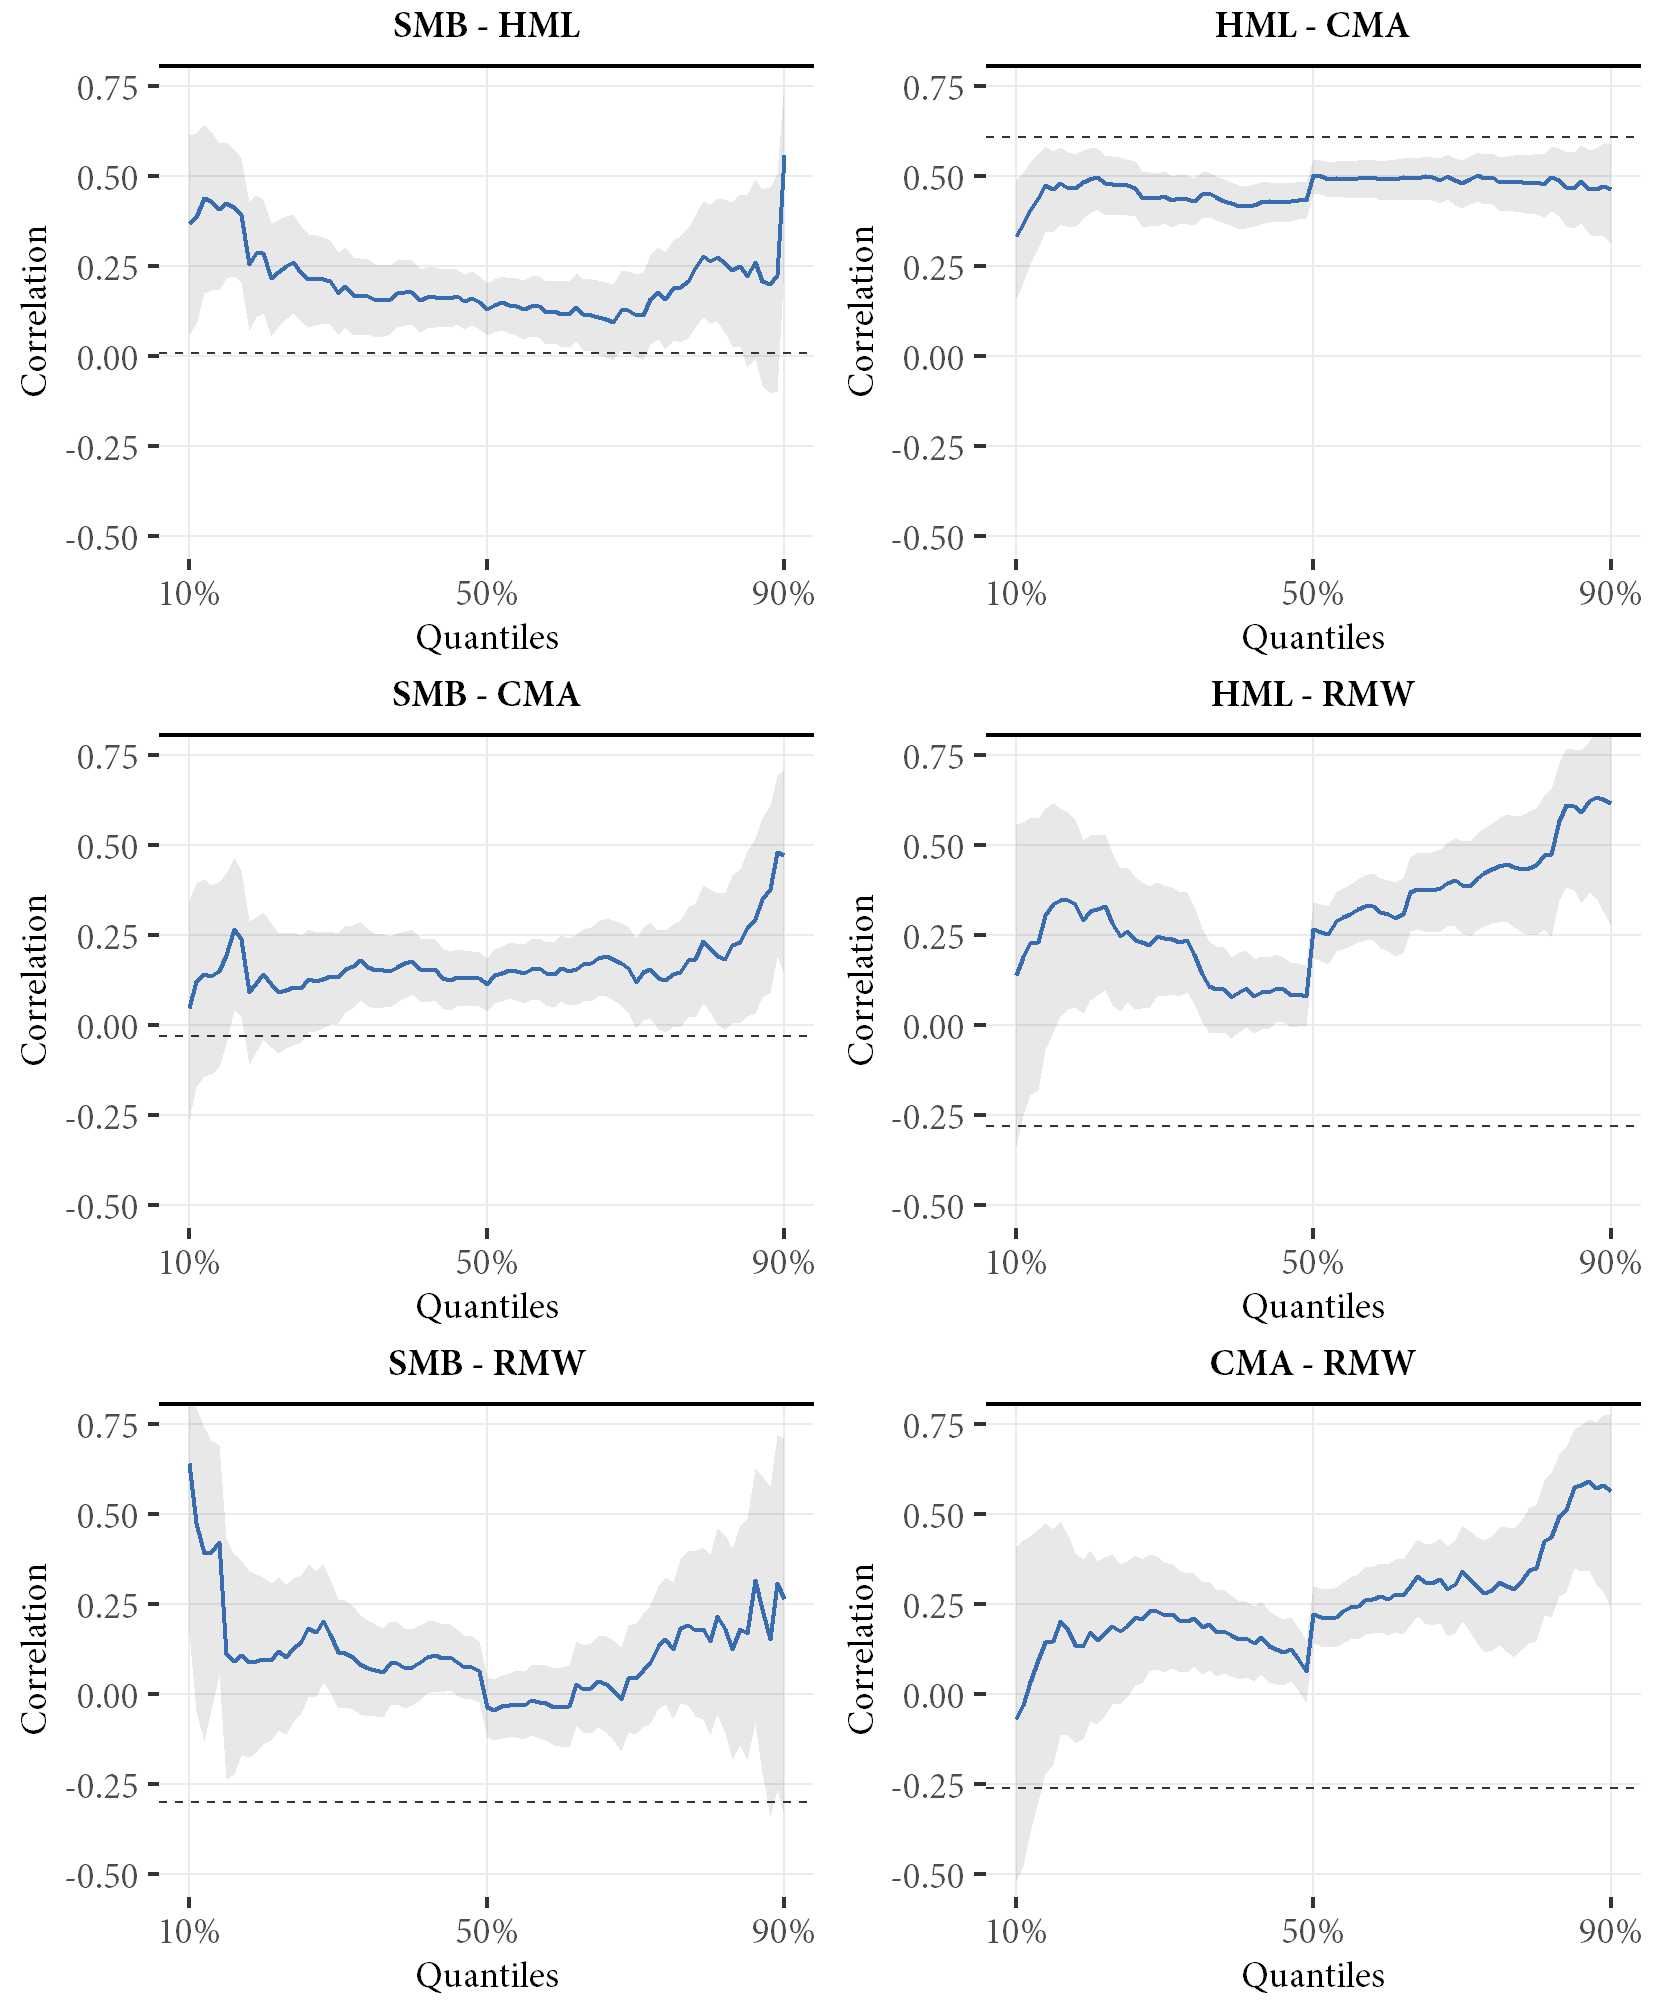
\includegraphics[scale=1]{graphics/threshold2.png}  
  %\bottomrule
  \vspace{3mm}
  \footnotesize
  Threshold correlation plots with 95\% confidence bounds. Correlation pairs in graph titles. Unconditional correlation given by the dashed line. Weekly ARMA-GARCH residuals from the chosen models, all data 1963-2016
  \end{minipage}
\end{figure}

% talk
As previously noted, we use residuals from the ARMA-GARCH models in the threshold correlation analysis instead of returns directly, as the residuals are sanitized of effects that can be explained on the univariate level alone. The plots for the standardized residuals are presented in~\autoref{fig:threshold1} and \autoref{fig:threshold2}. The patterns of returns and residuals are highly similar, with returns exhibiting more extreme patterns (see \autoref{app:threshold_return} for a comparison).

First, we note that the threshold correlation is significantly different from the unconditional correlation coefficient denoted by the dashed line for most factor pairs (with the exception of Mkt-RF - RMW, and CMA - HML). This means that the multivariate dependence of factor strategies has tail dependence that is not well captured by the standard correlation measure. Conditional on being in the first or third quadrant of returns, assuming a correlation coefficient of the unconditional correlation is misleading. A concrete example is provided by the Mkt-RF and HML pair. In a period when both residuals are observed below their 25\% percentile, the correlation is most certainly not -0.30, but actually positive.

In our multivariate analysis, we would like a model of joint returns to capture this behavior. Risk management is inherently a concern about what happens in the extremes, and the multivariate model should capture some of the tail dependence we observe in threshold correlations.

Second, we note that there is asymmetry around the median for some factor pairs, including the Mom - CMA, RMW - HML, RMW - CMA, and to a lesser extent Mkt-RF - RMW asset pairs. For example, in the Mom-CMA asset pair, the threshold correlation jumps up for the first percentile below the median, indicating that the correlation is higher when both realize below the median than when both realize above the median. This type of asymmetric property, where downside (below the median) correlation is higher than upside correlation is unwanted, as it reflects a poorer diversification in bad times. A good model of joint returns in factor strategies should therefore have flexibility to generate this type of asymmetry.

Third, we note that, although estimated with substantial uncertainty, the threshold correlation do not seem to be constant as $p$ approaches either zero or one. For example, the Mkt-RF - HML asset pair seems to have a downward pattern, where correlation is the most positive in the lowest percentiles of residuals and the most negative in the highest percentile of residuals. In fact, this pattern is unwanted from a diversification perspective, as diversification benefits decrease when the series are realizing in the lowest percentiles.

Fourth, while all other asset pairs exhibit unconditional correlations of around zero or negative, the CMA - HML pair exhibits high and positive correlation of more than 0.60. Furthermore, the threshold correlation estimate is much closer to the unconditional correlation. While all other factor strategy pairs appear to be very good diversifiers, CMA and HML factors look quite similar.

\subsection{Rolling correlation}
\label{subsec:roll_corr}
% method
We compute rolling correlation estimates in order to investigate whether the factor strategies exhibit constant correlation over time. 
\begin{align}
    RCorr(r_{i, t}, r_{j, t})_t^{w} = \frac{\sum^{t}_{t-w+1}(r_{i, t} - \bar{r}_i)(r_{j,t} - \bar{r}_j)}{\sqrt{\sum^{t}_{t-w+1} (r_{i,t} - \bar{r}_i)^2} \sqrt{\sum^{t}_{t-w+1} (r_{j,t} - \bar{r}_j)^2}}
\end{align}
where $r_i$, $r_j$ are the $N \cdot (N-1) / 2$ different pairs of the factor strategies' ARMA-GARCH residuals or log returns and $w$ is the rolling window of data. We use one year of data with $w = 52$ on weekly data. As previously, we use residuals from the ARMA-GARCH models in the rolling correlation analysis instead of returns directly and present results in~\autoref{fig:rolling1} and \autoref{fig:rolling2}.\footnote{A comparison of rolling correlations on returns and residuals is available in~\autoref{app:rolling_return}.}
% plots
\begin{figure}[H]
  \caption{Rolling correlations on ARMA-GARCH residuals. Page 1/2}
  \label{fig:rolling1}
  %\toprule
  \centering
  \begin{minipage}{\textwidth}
  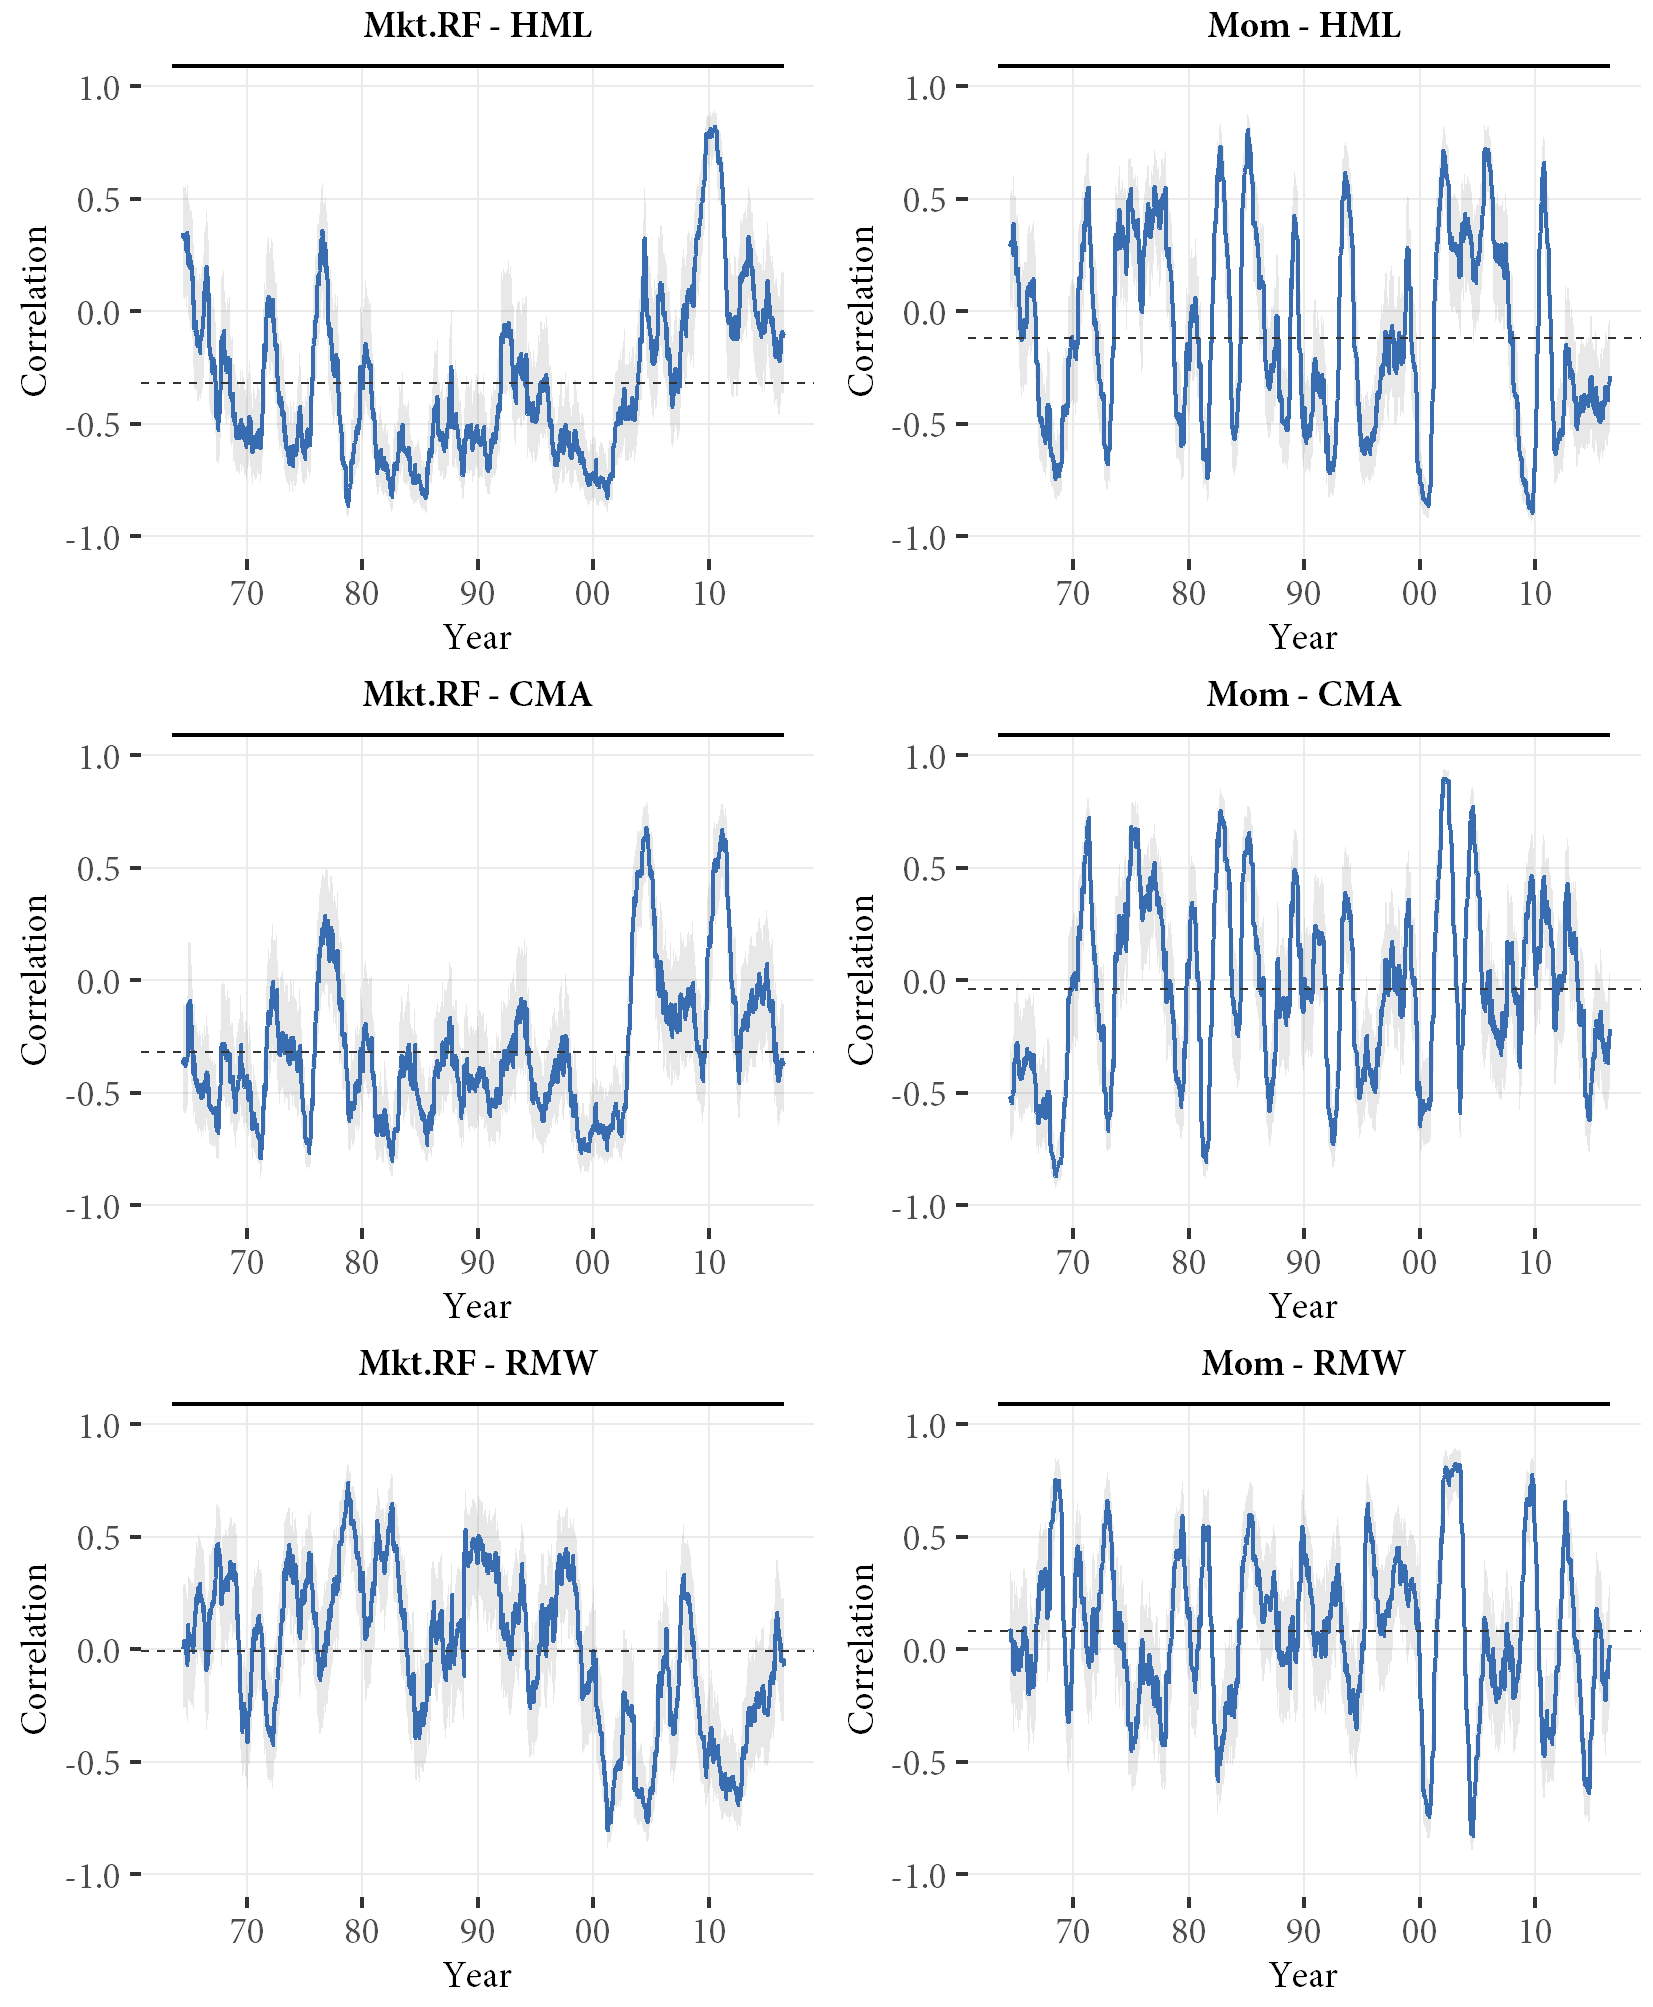
\includegraphics[scale=1]{graphics/rolling1.png}  
  %\bottomrule
  \vspace{3mm}
  \footnotesize
  Rolling correlation plots with 95\% confidence bounds. Correlation pairs in graph titles. Unconditional correlation given by the dashed line. Weekly ARMA-GARCH residuals from the chosen models, all data 1963-2016
  \end{minipage}
\end{figure}
\begin{figure}[H]
  \caption{Rolling correlations on ARMA-GARCH residuals. Page 2/2}
  \label{fig:rolling2}
  %\toprule
  \centering
  \begin{minipage}{\textwidth}
  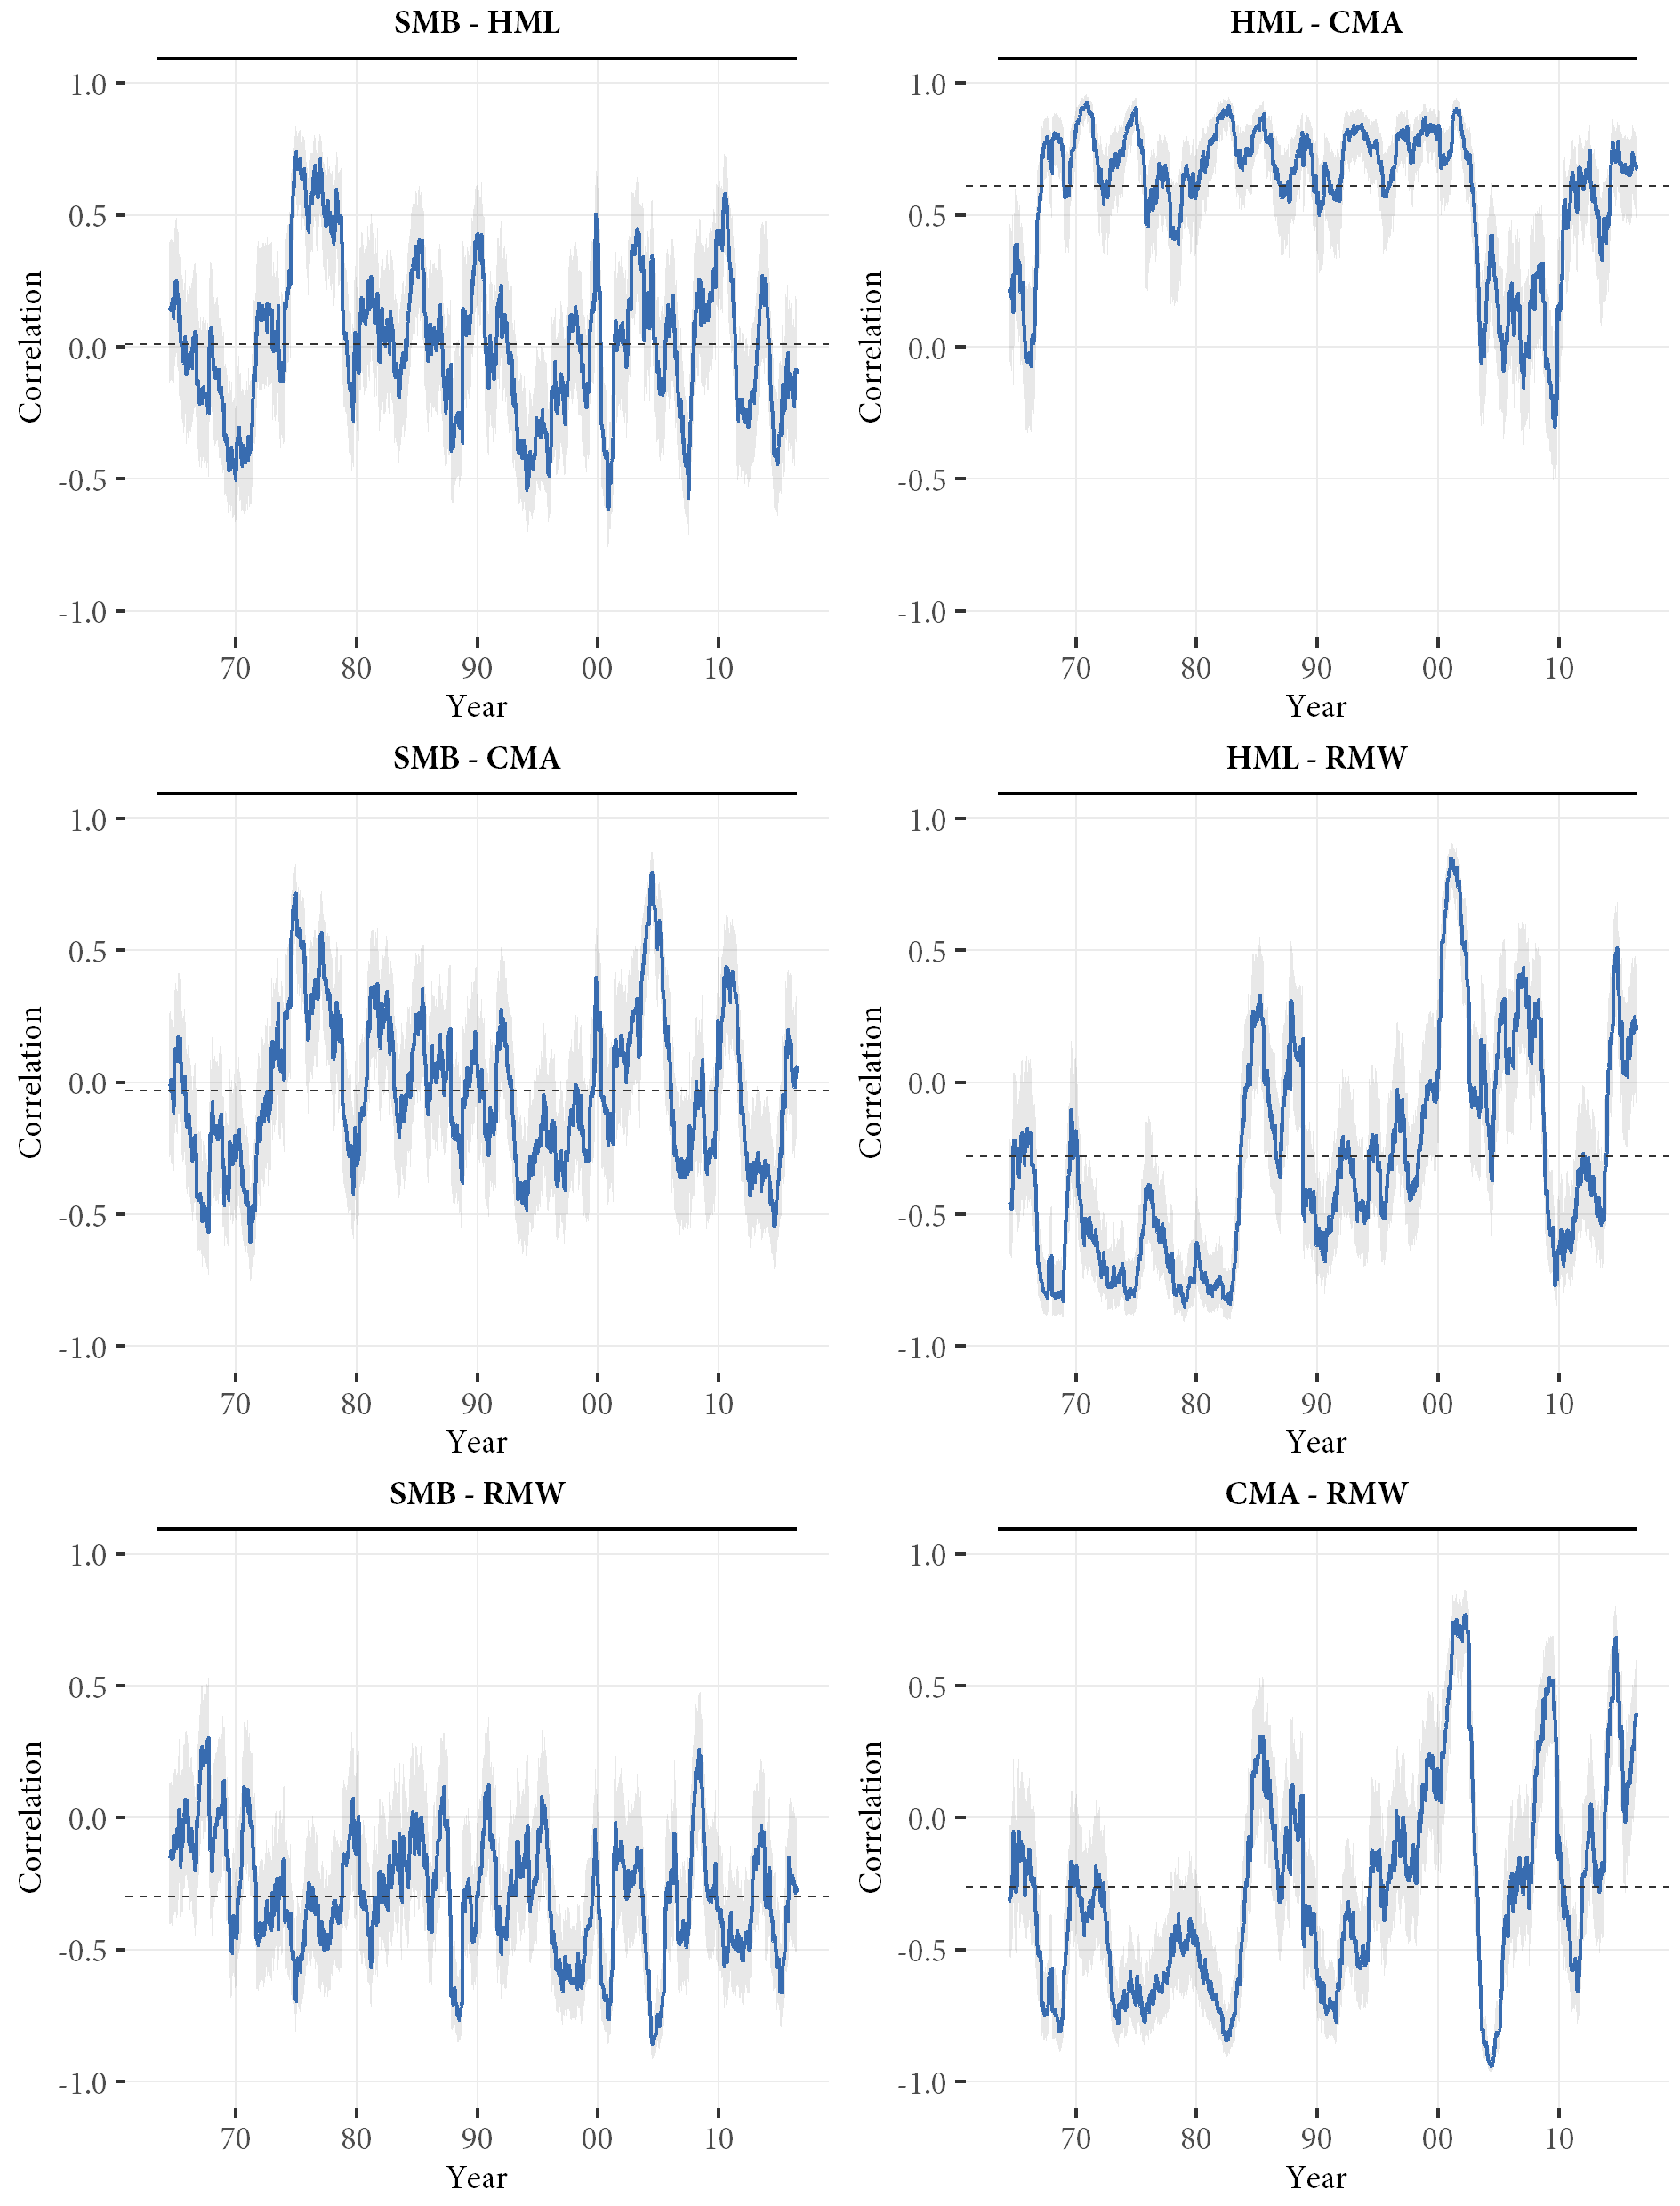
\includegraphics[scale=1]{graphics/rolling2.png}  
  %\bottomrule
  \vspace{3mm}
  \footnotesize
  Rolling correlation plots with 95\% confidence bounds. Correlation pairs in graph titles. Unconditional correlation given by the dashed line. Weekly ARMA-GARCH residuals from the chosen models, all data 1963-2016
  \end{minipage}
\end{figure}
% talk
First, we note that for most factor pairs, the rolling 52-week correlations are highly time-varying. While the unconditional correlation is often around zero, the rolling 52-week correlation ranges between approx. -0.75 and 0.75 for the HML - Mkt-RF factor pair. The time-varying correlations lead us to believe that a suitable model of joint returns will incorporate dynamic correlations. As long as there is some persistence in the series, a dynamic model should have merits in modeling returns jointly, as the best guess of tomorrow's correlation then is not simply the unconditional correlation.

Second, by visual inspection, the correlations of a few asset pairs could be suspected to be non-stationary, either due to overall trending or break points -- for example, the HML - Mkt-RF and CMA - HML asset pairs might have a break point around year 2000, as correlations are higher after this period; and the HML - CMA asset pair might have a break point around the same time, as correlations move outside a relatively close range of 40-90\% to substantially lower levels during 2000-2010. If trends or breakpoints were shown to be present, they could be incorporated in the model of joint returns. We believe that especially the potential upward trend in HML - Mkt-RF and CMA - Mkt-RF is highly interesting, and could mean that diversification benefits of these pairs is becoming weaker, but do not explore this further. In our model, we consider correlations to be stationary.

Third, the HML and CMA factors again stand out as different to other asset pairs. The unconditional correlation is much closer to the rolling estimates than for other factor pairs. However, while the correlation is quite high and constant for much of the early sample period, the lower correlations towards the end give reasons to think that they might in fact provide strong diversification benefits during certain times.

\subsection{Conclusions from analysis of multivariate dependence in univariate residuals}
Univariate residuals appear to be white noise series with no serial correlation or ARCH effects. However, there exists important dependence between residuals of different strategies. First, threshold correlations show that there is tail dependence -- in times when factor pairs simultaneously realize in their best and worst percentiles, correlations are significantly different from the unconditional mean. In fact, threshold correlations are substantially higher than the unconditional mean, which indicates that diversification benefits are smaller than expected when factors simultaneously have low returns. Second, rolling correlations show that correlations between series are highly time-varying and seem to exhibit persistence. This should mean that a dynamic model of correlations will improve on the description of joint returns.

Both analyses also show that the HML - CMA asset pair is quite different from the other pairs, exhibiting a much higher and more stable dependence. Differently put, they look quite similar as opposed to any other factor pair, and the merit of including both in factor portfolios seems more unclear.

For modeling of multivariate dependence, we expect that good candidate models will incorporate both tail dependence and dynamic correlations.